\documentclass{article}

\usepackage[dutch]{babel}
\usepackage[version=3]{mhchem} 
\usepackage{hyperref}
% Package for rendering imagnes better
\usepackage{pdfpages}
% Package import images
\usepackage{graphicx}
% Package for chancing the layout geometry
%\usepackage[margin=1in,includefoot]{geometry}

\usepackage{marvosym}
\usepackage{url}

%\usepackage{geometry}
\begin{document}

\title{\huge{Inrichting Centrale bank} }
\author{Merijn Plagge \\ 0941200}

\maketitle

\begin{abstract}

Voor project 4 moesten wij voor het individuele onderdeel een advies geven over het \emph{efficient inrichten van de Centrale Bank}.
Aan het eind van het eerste deel van het project moet \'e\'en van de adviezen van de studenten worden gekozen en uitgewerkt de rest van de loop van het project.
Wij moeten tijdens de loop van het project letten op vijf onderdelen: \emph{beheren, analyseren, adviseren ontwerpen en realiseren.}

\end{abstract}

\newpage

\tableofcontents

\newpage

\section{Opstelling en beheer project}

\subsection{Kwaliteitseisen}

Wij hebben een document met kwaliteitseisen voor de groep van de code, bank, ATM voor de groep.
Deze is op Github terug te vinden.
Ook individueel heb ik kwaliteitseisen voor de centrale bank opgesteld.
Al mijn individuele eisen heb ik toegepast in dit verslag.
De eisen van de groep gaan meer over de automaat, en hier zijn dus maar een paar punten van verwerkt. \\

\vspace{1mm}
\Mundus~\href{https://github.com/Gewad/Project4Bankalicious/blob/test/eisenlijstje.pdf}{Kwaliteitseisen team}

\Mundus~\href{https://github.com/Gewad/Project4Bankalicious/blob/merijn-branch/opdrachten/kwaliteitseisen/merijn/*.pdf}{Kwaliteitseisen individueel}

\subsection{Beheer}

Voor dit onderdeel moesten wij kunnen werken met Git en Version control.
Hier heb ik veel onderzoek over gedaan zodat ik dit goed kan toepassen dit project.
In figuur \ref{fig: git model} is het model wat wij gebruiken op onze Git pagina, \href{https://github.com/Gewad/Project4Bankalicious}{Project4Bankalicious}.
Ieder groepslid werkt op zijn individuele branch, en als je klaar bent met jouw onderdeel, dan wordt hij in test gemerged.
Als er geen problemen lijken te zijn op de test beslissen wij in een groep of wij test naar de master kunnen schrijven.
Al mijn en de groep's documentatie is terug te vinden op Github.

\begin{figure}[!h]
        \centering
        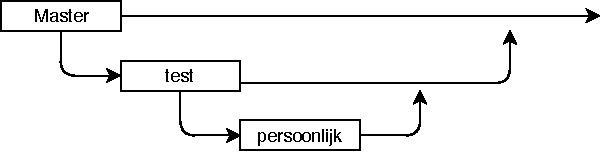
\includegraphics[height=0.7in]{git.pdf}
        \caption{git model}
        \label{fig: git model}
\end{figure}

\paragraph{Risico's en issue's}

Ik heb aan het begin van het project een risicolog opgesteld en door de loop van het project bijgehouden.
Deze is op de Gitpagina te vinden, en op mijn website. \\

\vspace{1mm}

\Mundus~\href{https://github.com/Gewad/Project4Bankalicious/blob/test/opdrachten/opdracht_h/opdracht_h_merijn/opdracht_h.pdf}{Risicolog persoonlijk}

\Mundus~\href{https://github.com/Gewad/Project4Bankalicious/blob/test/opdrachten/opdracht_h/opdracht_h_teamonderdeel.xlsx}{Risicolog team}

\paragraph{Issue tracking}

Op git houden wij individuele en persoonlijke issues bij.
Wij hebben hier een template voor gekregen, maar Git heeft dezelfde en meer mogelijkheden, en is overzichtelijker.
Bij de issues staan ook dingen die nog moeten gebeuren. \\ 

\vspace{1mm}

\Mundus~\href{https://github.com/Gewad/Project4Bankalicious/issues}{Git issues}

\newpage

\section{Communicatie}

\subsection{Server of servers?} 

Er zijn kort gezegd twee opties om de server(s) op te zetten.
Of wel \'e\'en centrale server, of meerdere losse servers die met elkaar praten.
Hieronder zal ik uitleggen welke ik gekozen heb en waarom.

\subsubsection{Verbonden servers}

Het veiligste idee is om meerdere servers te hebben.
Als een van meerdere servers uit zou vallen, zou het systeem nog steeds werken.
Ook is dit systeem schaalbaar, je kan de ballast van de ATM's verdelen over de servers.
De servers moeten de database gegevens met elkaar synchroniseren.
Elke update van een database zou via een query moeten doorgestuurd naar de andere database.
Omdat wij echter geen twee server locaties ter beschikking hebben voor het project is dit geen handig idee.

\begin{figure}[!h]
        \centering
        
\includegraphics[height=0.4in]{meerdere_servers.pdf}
        \caption{Meerdere servers}
        \label{fig: meerdere servers}
\end{figure}

\subsubsection{Centrale server}

Dit is het makkelijkste systeem.
Je hoeft namelijk maar \'e\'en server op te zetten.
De centrale bank zal communiceren met alle lokale ATM's.
De ATM's zullen om data vragen, en de server zal hierop reageren.
Ik wil alleen linux server van school wil gaan gebruiken, en het is dus niet praktisch om twee servers op \'e\'en locatie voor stroom te hebben.
Wel is het handig om een backup van de database te hebben op de server.
Ik stel voor om elk uur de database te encrypten, en in een aparte directory op te slaan.
Ik raad dit systeem aan voor de inrichting van de centrale bank.

\begin{figure}[!h]
        \centering
        
\includegraphics[height=0.4in]{centrale_server.pdf}
        \caption{Centrale server}
        \label{fig: centrale server}
\end{figure}

\newpage

\subsection{Protocol}

Er moet een protocol zijn om netjes op volgorde (met een queue), en programeertaalonhafhankelijk data te versturen over het netwerk.
Wij hebben over twee protocollen les gehad van docenten, en ik zal een van deze twee kiezen in mijn advies.

\subsubsection{MQ}

Message queueing werkt met een \emph{consumer} een een \emph{producer}.
De producer zal eerst een queue aan berichten maken, die de zogenaamde \emph{message broker} bijhoudt.
Als de producer klaar is met zijn lijst van berichten, ofwel batch genoemd, zal de broker deze een \emph{topic} geven en naar de consumer sturen.
Als echter tien ATM's allemaal een batch tegelijk naar de server sturen, zal de server misschien niet snel genoeg zijn om dit in een keer te verwerken.
Ook is het niet nodig om met een batch te werken, omdat je niet heel veel data in een keer hoeft te sturen.
Als een ATM 100 euro opvraagt, dan is dat maar een message.
De enige keer dat dit practisch is, is bij het versturen van de pincode en de RFID code tegelijkertijd.
Maar dit zou ook in twee messages gedaan kunnen worden.
Daarom raad ik dit protocol niet aan.

\subsubsection{MQTT}

MQTT werkt in tegenstelling van MQ niet met batches, maar met enkele messages, en is dus erg licht.
De server kan dus sneller berichten verwerken.
Het werkt in plaats van met batches met subscriptions.
De publisher stuurt berichten naar de server, en de subscribers kiezen wat ze hier mee doen.
De subscriber kan uit drie opties kiezen.
Deze niveaus heten \emph{Quality of Service}.
Ik raad dit protocol aan omdat het lichter is dan MQ, zodat de server niet overbelast raakt.
Voor het bank project hebben wij QoS-2 nodig, omdat je anders per ongeluk bijvoorbeeld twee keer hetzelfde bedrag kan afschrijven.

\begin{description}
\item [QoS-0:] Een keer sturen, en niet kijken of het bericht is aangekomen.
\item [QoS-1:] Minstens een keer sturen, en kijken of het bericht is aangekomen.
\item [QoS-2:] Een keer sturen, en een keer ontvangen.
\end{description}

\newpage

\section{Encryption}

\subsection{Analyze en advies beveiliging netwerk} 

Er zijn redelijk wat opties voor beveiliging voor netwerkverkeer.
Veel protocollen zijn onveilig verklaart.
Ik zal uitleg geven welke problemen hebben, en welke wel te gebruiken voor de bank.

\subsubsection{Problemen geen netwerk encryption}

Als er op het netwerk geen encryption zou zitten zouden er verschillende zwakke plekken zijn in het beveiligingssysteem.
Zo kan bijvoorbeeld zonder protocol de verbinding niet alleen worden afgeluisterd, maar zou een hacker zich ook voor kunnen doen als een server.

\subsubsection{SSL tot TLS}

SSL en TLS zijn protocollen voor de communicatie security tussen de client en server.
Als dit protocol gebruikt wordt is het communicatieverkeer niet zo maar af te luisteren.
Er is echter grote problemen met SSL, er zijn veel aanvallen die je makkelijk over een versleuteld netwerk kunt uitvoeren, zoals de een POODLE attack.
Deze attack komt er op neer dan als een aanvaller genoeg request stuurt naar de server of de client, hij de encryption kan kraken.
Dit probleem komt voor in SSL1, SSL2, en SSL3.

Ook in TLS, die opvolger van SSL, zijn in oude versies al kwetsbaarheden gevonden om de encryptie te kraken.
SSL en TLS zijn protocollen voor de communicatie security tussen de client en server.
Als dit protocol gebruikt wordt is het communicatieverkeer niet zo maar af te luisteren.

Sinds juni 2018 zijn alle SSL protocollen verboden te gebruiken voor organisaties die vallen onder het PCI DSS (Payment Card Industry Data Security Standard).
Nieuwe versies zoals TLS 1.1 en TLS 1.2 mogen nog wel hiervoor worden gebruikt.
Ik raad aan om ons banksysteem ook aan deze regelgeving te houden, en TLS 1.2 te gebruiken.

\newpage

\subsection{Analyze en advies beveiliging lokale opslag} 

Hieronder zijn verschillende manieren te vinden hoe inloggegevens en andere gevoelige informatie op kunnen worden geslagen.
Ik heb het hier over de voor en nadelen van deze manieren, en ook geef ik hier advies of het van toepassing is bij de bank.

\subsubsection{Plain text}

Dit is de meest onveilige manier om wachtwoorden, pincodes, RFID-codes op te slaan.
Stel je database raakt op de een of andere manier blootgesteld aan onbevoegden personen, dan kan je makkelijk pincodes en RFID-codes aflezen. 
Het is wel de makkelijkste manier om inloggegevens op te slaan.
Je kan namelijk makkelijk alle gegevens opvragen zonder moeite.

Maar sinds het hier om de beveiliging van een bank gaat is dit niet veilig genoeg.
Tijdens het ontwikkelen van de centrale bank zou het wel tijdelijk kunnen worden toegepast om onderdelen te testen, en zou daarna vervangen moeten worden door een ge\"encrypt systeem.

\subsubsection{Encrypt de hele database}

Een andere veiligere optie is om de database lokaal te versleutelen.
Stel de gebruiker stuurt een pincode naar de server, dan decrypt de server die pincode in de database, en vergelijkt de pincodes.
Een encryptie algoritme zoals AES of DES zijn voor dit project geschikt, omdat het in veel programeertalen beschikbaar is.
Dit is nodig omdat sommige groepjes misschien in andere talen hun bank willen schrijven.
Een keysize van 64 bit is genoeg, omdat het zo ongeveer 550 jaar kan duren om dit te ontsleutelen.
AES werkt op het laagste niveau met 128 bits, wat te veel is.
Je levert snelheid in als je te veel bits gebruikt.
DES kan met 64 bit werken, en deze raad ik aan om te gebruiken.

Dit is al een stuk veiliger dan een plain text wachtwoord, maar het heeft nog steeds een nadeel.
Als een hacker de key om de database te ontsleutelen te pakken krijgt, dan kan hij alle wachtwoorden achterhalen.
Ook zullen dezelfde wachtwoorden zichtbaar zijn, omdat de ge-encrypte wachtwoorden er hetzelfde uitzien.

Mijn advies is om ook dit systeem niet te gebruiken, al is het een stuk veiliger dan plain text.
Het zou voor een schoolprojectje goed genoeg zijn, sinds zelfs grote bedrijven deze fouten nog maken, maar het is beter om de later beschreven manieren te gebruiken.

\newpage

\subsubsection{Hashing}

Naast de hele database te versleutelen kan je ook de individuele pincodes and RFID codes hashen.
Het verschil tussen een hash en een ge-encrypte string is dat je een hash niet terug kunt zetten naar het origineel met een key. 
Een hash kan je wel zelf terugrekenen.
Naast de hele database te versleutelen kan je ook de individuele pincodes and RFID codes hashen.
Het moet een langzame hashing methode zijn omdat je anders als hacker snel wachtwoorden zou kunnen raden.
Een goed algoritme hiervoor zou SHA1 kunnen zijn.
Md5 is hier bijvoorbeeld niet voor geschikt omdat het erg snel is.
Sinds SHA1 in veel talen beschikbaar ik, adviseer ik deze te gebruiken.
Het moment dat de gebruiker bijvoorbeeld een pincode invoert, zal deze gehashed worden.
Zodra deze bij de database aankomt zullen de hashes worden vergeleken.
Dit is veiliger dan de hele database te encrypten, omdat de gegevens niet meer decrypt hoeven te worden.
Je hebt jammer genoeg nog steeds het probleem dat je versleutelde data met elkaar kunt vergelijken.
Gebruikers met hetzelfde wachtwoord zullen ook dezelfde hash hebben.
Je hebt ook zogenaamde rainbow tables.
Dit zijn tabellen waar mensen de hashes al voor je hebben uitgerekend.
Zo kan je ook snel door de meer zware hashing algoritmes heen gaan, en zijn deze ook niet veilig.

\hfill

\centerline{\ce{pincode ->[hash] hashed} \ce{pincode} }

\newpage

\subsubsection{Hashing and Salting}

De beveiligingsproblemen die overblijven bij hashen zijn op te lossen, waarna geen beveiligingsproblemen overblijven met de database.
Ze zijn op te lossen door midden van \emph{Salting}.
Ik raad dan ook aan om dit systeem te gebruiken voor de beveiliging.
Dit is een voor iedere gebruiker random gegenereerde string die je opslaat in de database.
Het idee is om gevoelige gegevens, als ze worden ingevoerd aan deze string te koppelen, waarna je ze door een hashing algoritme stuurt.
Het resultaat sla je op in je database.
Als de gebruiker een pincode invoert dan zal eerst de pincode ge-encrypt moeten worden.
Dit moet in de Arduino gebeuren sinds data tussen de computer en Arduino kan worden afgeluisterd.
Hierna zal een een session based hash worden gebruikt om de data nog meer te versleutelen.
Dit wordt gedaan omdat je als hacker magnetische straling kan opvangen van de Arduino.
Als een hacker genoeg data weet te verzamelen kan hij je encryptie kraken als je geen session based systeem hebt.
Hier wordt geen hashing gebruikt die ook op de server wordt gebruikt omdat je anders weet hoe de server wachtwoorden vergelijkt in de database.
Hierna stuurt de Arduino deze string via de computer naar de server.
Op de server zal de binnenkomende pincode gedecrypt worden.
Hierna zal de salt worden toegevoegd, en zal de string worden gehashed.
Dan wordt de hash vergeleken met de hash in de database.

Hieronder is visueel weergegeven wat mijn model is om een pincode veilig te vergelijken naar de database te krijgen. De laatste hash zal vergeleken worden met de hash in de database.
Als de server een command terug stuurt, zal simpelweg het command encrypten, en daarna hashen met de sessionhash.

\hfill

\centerline{\textbf{Arduino to server} \ce{pin ->[\textbf{Arduino}\ encrytion] encrypted ->[Session hash] hashed ->[\textbf{Server}\ decryption]}}

\vspace{1cm}

\centerline{\textbf{Op de server} \ce{pin ->[salting] pin $+$ salt ->[hashing] hash ->[Vergelijk\ me\ hash\ database] Klopt\ wel\ of\ niet}}

\vspace{1cm}

\centerline{\textbf{Saldo naar Arduino} \ce{Saldo ->[\textbf{server}\ encryption] string ->[Session hash] hashed ->[\textbf{Arduino}\ decryption]}}

\end{document}


